% \documentclass{article}
\documentclass{ctexart}

\usepackage{graphicx}
\usepackage{amsmath}
\usepackage{amssymb}
\usepackage{amsthm}
\usepackage{BOONDOX-cal}
\usepackage{subfigure}
\usepackage{url}
\usepackage{float}
\CJKfamily{song}
% \setCJKfamilyfont{song}
\CTEXsetup[format={\Large\bfseries}]{section}

\usepackage{tikz}
\usetikzlibrary{positioning, shapes.geometric}

\usepackage{listings}
\usepackage{color,xcolor}
\setlength{\parindent}{0pt}

\title{作业六:一元二次方程在实数域上的解}


\author{常笑 \\ 数学与应用数学 \\ 3190102223 }

\begin{document}

\maketitle

\section{理论}
\indent 对于一个一元二次方程 $ax^2 + bx + c = 0,(a \neq 0) $,我们可以对其配方,作如下等价变换:
\begin{equation}
   \indent ax^2 + bx + c = 0 \\
   \iff a(x + \frac{b}{2a})^2 + c - \frac{b^2}{4a} = 0\\
   \iff (x + \frac{b}{2a})^2  = \frac{b^2}{4a^2} - \frac{c}{a}\\
\end{equation}
\indent 由此我们知道该一元二次方程在实数域上的解有三种情况
\subsection{$\frac{b^2}{4a^2} - \frac{c}{a} < 0$}
\indent 由于等式左式是大于等于$ 0 $的,而右式却小于 $0$,矛盾,方程没有解,对应的图像如下:
\begin{figure}[h]
\centering
\subfigure[\label{1} a < 0]
{
    \begin{minipage}[b]{.45\linewidth}
        \centering
        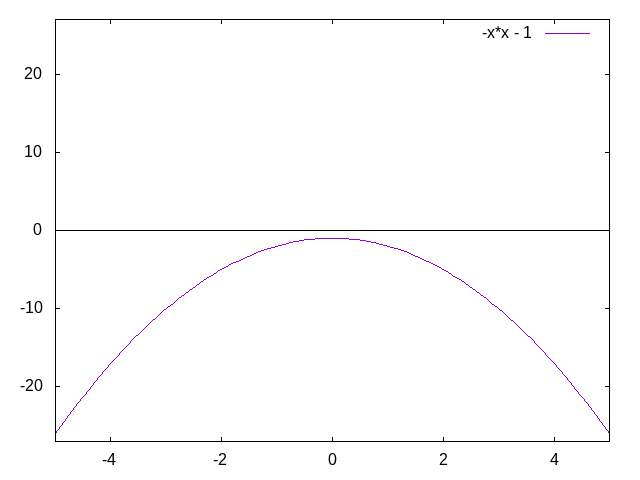
\includegraphics[width=5cm]{./examples/none_n.png}
    \end{minipage}
}
\subfigure[\label{2} a > 0]
{
   \begin{minipage}[b]{.45\linewidth}
        \centering
        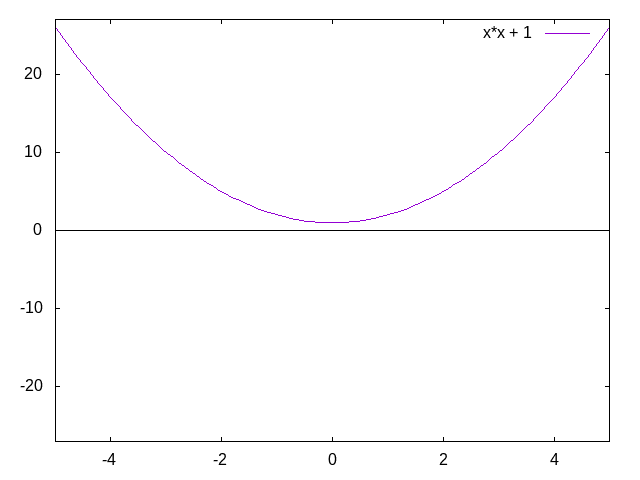
\includegraphics[width=5cm]{./examples/none_p.png}
    \end{minipage}
}
\caption{}
\end{figure}

\subsection{$\frac{b^2}{4a^2} - \frac{c}{a} = 0$}
\indent 可知这时在实数域上有二重根$x = -\frac{b}{2a}$,对应的图像如下:
\begin{figure}[h]
\centering
\subfigure[\label{1} a < 0]
{
    \begin{minipage}[b]{.45\linewidth}
        \centering
        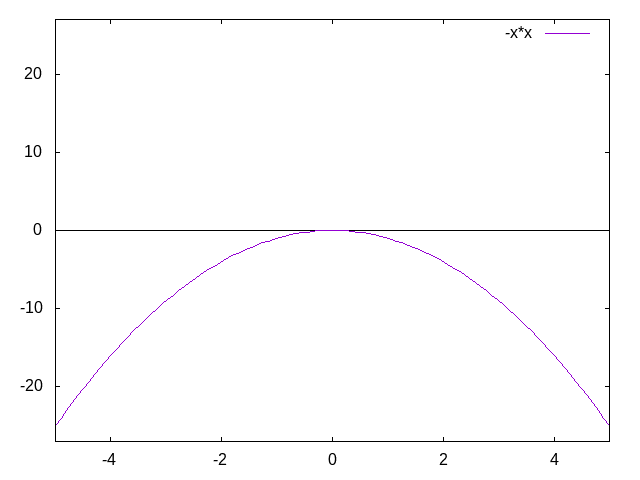
\includegraphics[width=5cm]{./examples/one_n.png}
    \end{minipage}
}
\subfigure[\label{2} a > 0]
{
   \begin{minipage}[b]{.45\linewidth}
        \centering
        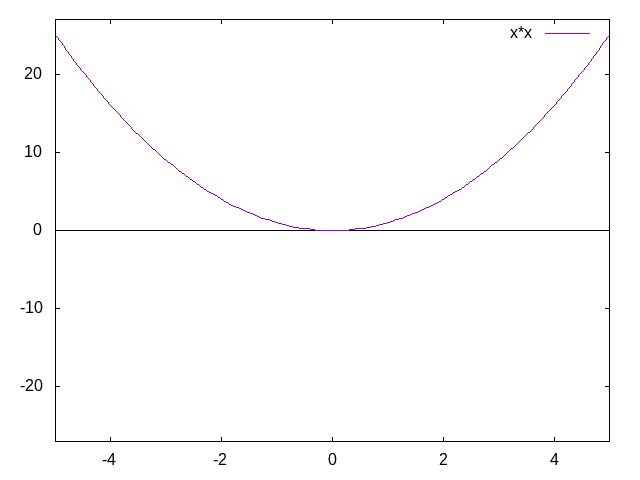
\includegraphics[width=5cm]{./examples/one_p.png}
    \end{minipage}
}
\caption{}
\end{figure}

\subsection{$\frac{b^2}{4a^2} - \frac{c}{a} > 0$}
\indent 可知这时在实数域上有二个根$x_1 = \frac{-b - \sqrt{b^2 - 4ac}}{2a} ,x_2 =\frac{-b + \sqrt{b^2 - 4ac}}{2a}$,对应的图像如下:
\begin{figure}[h]
\centering
\subfigure[\label{1} a < 0]
{
    \begin{minipage}[b]{.45\linewidth}
        \centering
        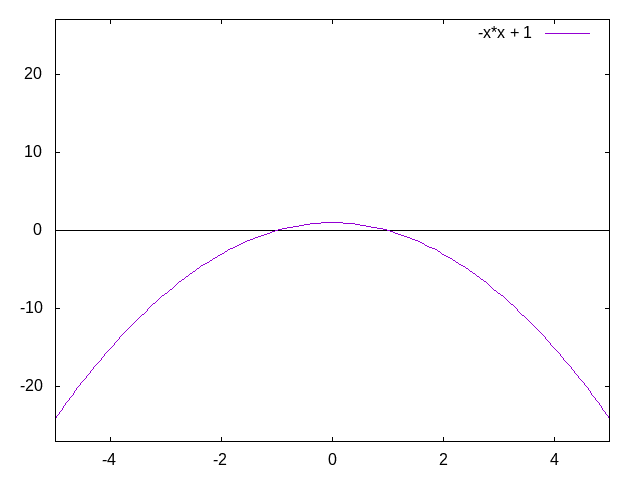
\includegraphics[width=5cm]{./examples/two_n.png}
    \end{minipage}
}
\subfigure[\label{2} a > 0]
{
   \begin{minipage}[b]{.45\linewidth}
        \centering
        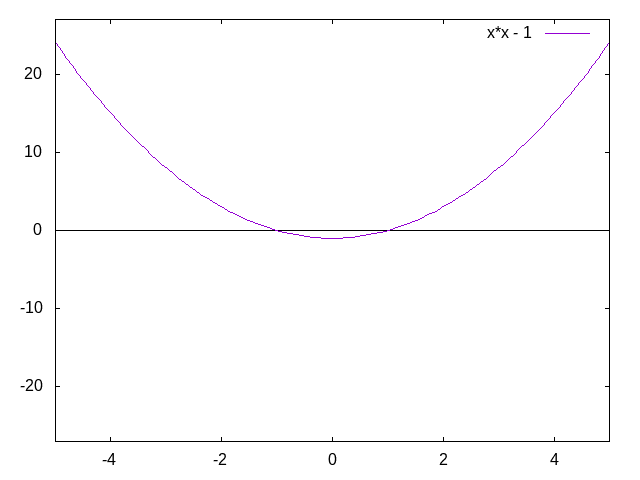
\includegraphics[width=5cm]{./examples/two_p.png}
    \end{minipage}
}
\caption{}
\end{figure}
\section{算法流程}
\indent 由上边理论推导过程,我们可以作出求解这样一个一元二次方程的流程图如下:

\begin{tikzpicture}[node distance=10pt]
  \node[draw, rounded corners]                        (start)   {得到输入a,b,c};
  \node[draw, diamond, aspect=3, below=of start]                         (judge)  {计算 $b^2 - 4ac$};
  \node[draw, rounded corners, below=20pt of judge]                        (cal1)  {输出两个根$x_1,x_2$};
  \node[draw, rounded corners, left=30pt of cal1]                   (cal2)  {输出二重根$-\frac{b}{2a}$};
  \node[draw, rounded corners, right=30pt of cal1]  (cal3)     {输出:该方程无实根};
  
  \draw[->] (start)  -- (judge);
  \draw[->] (judge) -- node[above] {$b^2 - 4ac < 0$} (judge -|cal3) -> (cal3);
  \draw[->] (judge) -- node[above]  {$b^2 - 4ac = 0$} (judge -|cal2) -> (cal2);
  \draw[->] (judge) -- node[left] {$b^2 - 4ac > 0$}  (cal1);
\end{tikzpicture}

\begin{figure}[h]
\centering

\end{figure}


\end{document}